 \documentclass[conference]{IEEEtran}
\IEEEoverridecommandlockouts
% The preceding line is only needed to identify funding in the first footnote. If that is unneeded, please comment it out.
%Template version as of 6/27/2024

\usepackage{cite}
\usepackage{amsmath,amssymb,amsfonts}
\usepackage{graphicx}
\usepackage{textcomp}
\usepackage{xcolor}
\usepackage{url}
\usepackage[capitalise]{cleveref}
\usepackage{booktabs}
\usepackage{threeparttable}
\usepackage{array}
\newcolumntype{L}[1]{>{\raggedright\arraybackslash}p{#1}}
\def\BibTeX{{\rm B\kern-.05em{\sc i\kern-.025em b}\kern-.08em
    T\kern-.1667em\lower.7ex\hbox{E}\kern-.125emX}}
\begin{document}
\bstctlcite{IEEEexample:BSTcontrol}

\title{Auditing SHAP Explanations Against Known Failure Mechanisms in Predictive Maintenance\\
% {\footnotesize \textsuperscript{*}Note: Sub-titles are not captured for https://ieeexplore.ieee.org  and
% should not be used}
% \thanks{Identify applicable funding agency here. If none, delete this.}
}

\author{\IEEEauthorblockN{Koshik Debanath, Prakrit Uprety, and Peiyu Li}
\IEEEauthorblockA{Department of Computer Science, South Dakota State University\\
Brookings, SD, USA\\
\{koshik.debanath, prakrit.uprety\}@jacks.sdstate.edu, peiyu.li@sdstate.edu}
}

\maketitle

\begin{abstract}
A failure-prediction model can be accurate and still base its predictions on the wrong inputs. We propose a statistical audit that checks, for each documented failure mechanism, whether held-out SHAP attributions concentrate on the features named in that mechanism's rule. The audit uses three statistics, which measure the share of attribution on these features, how much larger this share is than on other failures, and how much any other feature gains. Each statistic is compared with pipelines retrained on shuffled labels. On the AI4I 2020 benchmark, a tuned XGBoost classifier (test F1 = 0.89) passes the audit for three of four physical mechanisms. The tool-wear result depends on the reference distribution of the explanation. It fails with path-dependent TreeSHAP and passes when attributions are measured against normal operation. A planted shortcut sensor shows that accuracy can stay high while attribution moves to a misleading feature, and that weak shortcuts, or shortcuts spread over several sensors, go undetected. On laboratory bearing recordings and simulated Tennessee Eastman process data, the audit finds attribution consistent with the specified features for inner- and outer-race faults and a reactor-cooling fault, and it flags an injected acquisition-gain shortcut although classification accuracy remains perfect. A passing audit is evidence about where attribution falls under a given mechanism map. It does not certify that the model is physically correct, and flagged features need to be investigated.
\end{abstract}

\begin{IEEEkeywords}
Explainable AI, SHAP, predictive maintenance, feature attribution evaluation,
physical failure mechanisms
\end{IEEEkeywords}

\section{Introduction}
Predictive maintenance uses machine-condition data to anticipate faults and reduce unplanned downtime~\cite{cummins2024survey}. Explanation methods such as SHAP~\cite{lundberg2017shap} and LIME~\cite{ribeiro2016lime} are now common in this field, where they show maintenance teams which sensor readings drive an alarm~\cite{steurtewagen2021adding,gawde2024explainable,ndao2025improving}. For mechanism-based diagnosis, practitioners need to distinguish attribution to expected failure conditions from attribution to artefacts or downstream responses. A model may, for example, predict a heat-dissipation failure correctly because of an acquisition artefact in the data and pay little attention to temperature and rotational speed. High predictive performance and this kind of shortcut can occur together~\cite{geirhos2020shortcut,lapuschkin2019unmasking}.

In this paper we test, for each known failure mechanism, whether the model's attribution concentrates on the features that define the mechanism more strongly than the attribution of pipelines trained without any label signal. This requires two references. The first records which mechanism occurred and which features its rule uses~\cite{zhou2022attribute}. The second describes what attribution looks like when a model has learned nothing~\cite{altmann2010permutation}. Agreement with the mechanism features tells us how the model distributes its attributions under a stated mechanism map. It does not show that the model reasons causally~\cite{janzing2020feature}.

The AI4I~2020 dataset~\cite{uci2020ai4i} provides recorded mechanism indicators and documented generation rules. We also use laboratory bearing recordings (CWRU), in which each fault location has a known defect frequency, and simulated Tennessee Eastman process (TEP) data, in which each fault acts on a known cooling loop. Earlier explanation studies on AI4I examine selected examples, global rankings, or the agreement between explainers (\cref{sec:related}), but none tests mechanism-level attribution on held-out data against a statistical reference.

Our audit trains a classifier on the overall failure label only, explains held-out observations, groups the explanations by recorded mechanism, and compares three statistics with pipelines retrained on shuffled labels (\cref{fig:pipeline}). We study whether the audit rejects a model that has learned nothing and which design choices this requires, how its results change with the data, model, explainer, and reference distribution, how strong a planted shortcut has to be before the audit reacts, and how the audit behaves on measured and process data. The main contributions of this paper are as follows.
\begin{itemize}
    \item We formulate a mechanism-level audit with three attribution statistics computed on held-out explanations, a retrained shuffled-label reference, and a decision rule that labels each mechanism as aligned, flagged, or not aligned for a stated configuration.
    \item We study the behaviour of the audit in controlled experiments. Leaving out held-out explanations or the retrained reference led to misleading passes, a planted sensor went undetected when weak and was detected when stronger, and the tool-wear result changed with the attribution reference.
    \item We apply the audit to AI4I~2020, laboratory bearing recordings, and simulated process data, and provide an accompanying supplement and a versioned computational snapshot~\cite{artifact}.
\end{itemize}

\section{Related Work and Background}
\label{sec:related}

Surveys of explainable predictive maintenance cover interpretable models, surrogates, LIME, and SHAP~\cite{cummins2024survey,vollert2021interpretable}. Applications use Shapley values for breakdown diagnosis~\cite{steurtewagen2021adding}, compare LIME, SHAP, and attribute-wise explanations~\cite{jalali2020interpretability}, accelerate SHAP for fault diagnosis~\cite{chen2025shep}, or compare Integrated Gradients and SHAP on TEP~\cite{gravanis2026explainability}. Closest to our setting, Matzka~\cite{matzka2020explainable} checked explanations on AI4I~2020 against its known mechanisms with five examples per physical failure type; later work interpreted global SHAP rankings~\cite{milling2025shap} or measured SHAP--LIME agreement~\cite{obeten2026agreement}. These studies inspect individual examples or compare explainers with each other. They do not test attribution against a statistical reference.

SHAP assigns additive contributions relative to a baseline~\cite{lundberg2017shap}, and the way unavailable features are represented is part of what an explanation means~\cite{covert2021explaining}. Shapley variants condition on the remaining features, marginalize over a background, or substitute one baseline~\cite{sundararajan2020many}, and they answer different questions, especially for correlated inputs~\cite{chen2023algorithms,chen2020true,aas2021explaining,kumar2020problems}. Path-dependent TreeSHAP weights tree paths by their training cover, whereas interventional TreeSHAP averages over an explicit background~\cite{lundberg2020treeshap}; faster algorithms keep the path-dependent formulation~\cite{yu2022linear,wettenstein2026quadrature}, FastPD estimates partial-dependence-based SHAP consistently under correlation~\cite{liu2025fastpd}, and pairwise Shapley values use a single chosen reference~\cite{xu2025pairwise}. For gradient attributions, the baseline and the integration path play the same role~\cite{sturmfels2020visualizing}, and averaging over many baselines avoids relying on a single one~\cite{erion2021improving}. As \cref{sec:variants} shows, this choice can change the result for a mechanism, so an industrial audit has to state the reference it uses.

Ground-truth benchmarks test whether attributions recover planted relevance~\cite{liu2021synthetic,lee2025xaiunits,yang2019bam,arras2022clevr}, faithfulness metrics score explainers~\cite{agarwal2022openxai,li2024dual}, removal-based evaluations retrain or re-score without highly attributed inputs~\cite{hooker2019roar,rong2022road}, and HSIC measures input--output dependence without attribution~\cite{daveiga2015global}. Label permutations calibrate classifier accuracy~\cite{ojala2010permutation} and feature importance~\cite{altmann2010permutation}, and randomization tests expose saliency maps that ignore the model~\cite{adebayo2018sanity,kindermans2019unreliability}; explanations can also be manipulated~\cite{slack2020fooling}. Equally accurate models and different explainers can explain the same data differently~\cite{fisher2019all,black2022multiplicity,krishna2024disagreement}, so we report verdicts across seeds, references, models, and explainers. Selection-adjusted tests of global SHAP importance~\cite{kim2025phitest} ask which features matter for the model overall, whereas we ask whether the attribution on each recorded mechanism falls on that mechanism's features; the two are complementary. To our knowledge, none of these methods tests whether attribution on each recorded failure mechanism concentrates on that mechanism's documented features beyond a retrained shuffled-label reference.

\section{Methodology}
\label{sec:method}

\subsection{Problem Definition}
\label{sec:background}

Let $\mathcal{D}=\{(x_i,y_i,z_i)\}_{i=1}^{N}$, where $x_i\in\mathbb{R}^{d}$ holds the input features, $y_i\in\{0,1\}$ indicates overall failure, and $z_i\in\{0,1\}^{M}$ records $M$ failure mechanisms. A classifier $f$ is trained on $(x_i,y_i)$ only; the mechanism indicators are reserved for evaluating its explanations. For each mechanism $m$, domain knowledge fixes a set $E_m$ of \emph{expected} (trigger) features before the audit. Let $S_m=\{i:z_{i,m}=1\}$ be the \emph{mechanism-positive} observations, $F=\{i:y_i=1\}$ the observations labeled as failures, and $\phi_j(x_i)$ the SHAP attribution of feature $j$ for observation $i$.

Each audit result refers to one configuration, namely the pipeline, the attribution method and its reference distribution, the expected sets, and the evaluation sample. It describes the model's attributions for a mechanism under this configuration and says nothing about whether the mechanism itself is correct. A result of \emph{not aligned} (\cref{sec:nulls}) means that the test found insufficient evidence; it does not imply that the model reasons in a physically wrong way.

\begin{figure*}[t]
\centering
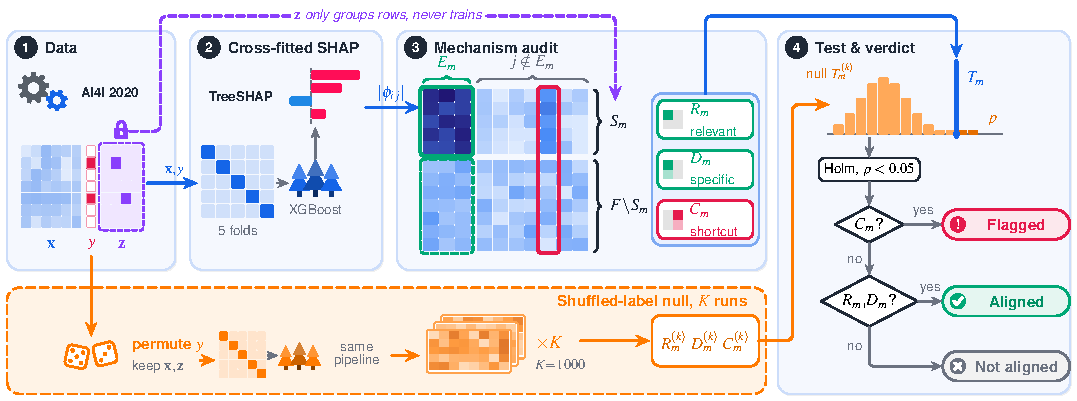
\includegraphics[width=\textwidth]{figures/audit_pipeline.pdf}
\caption{Mechanism-level SHAP audit. (1)~The classifier is trained on
$\mathbf{x}$ and the failure label $y$; the mechanism flags $\mathbf{z}$
only group observations, and the expected sets $E_m$ are fixed beforehand
from failure rules or physics. (2)~Five-fold cross-fitting gives every observation a
TreeSHAP explanation from a model that did not train on it. (3)~The
attributions $|\phi_{ij}|$ on $S_m$ and $F\setminus S_m$ give $R_m$, $D_m$, and
$C_m$: green marks $E_m$ (solid: $S_m$, giving $R_m$; solid versus dashed:
$D_m$), red the outside feature with the largest excess ($C_m$).
(4)~Each statistic is compared with $K$ shuffled-label refits (orange); after
Holm correction, a mechanism is flagged if $C_m$ is significant, aligned if
$R_m$ and $D_m$ are, and not aligned otherwise.}
\label{fig:pipeline}
\end{figure*}

\subsection{Dataset and Failure Mechanisms}
\label{sec:data}

AI4I~2020~\cite{matzka2020explainable} is a synthetic milling dataset of 10{,}000 observations. Each observation records product quality (\texttt{L}, \texttt{M}, \texttt{H}), air and process temperatures, rotational speed, torque, tool wear, an overall failure label (339 failures, 3.4\%), and five mechanism indicators for tool wear (TWF), heat dissipation (HDF), power (PWF), overstrain (OSF), and random failure (RNF). \Cref{tab:mechanisms} lists the documented rules and expected sets. The label is intended to be the OR of the indicators, but the mechanism-positive observations and the labeled failures are not the same set. Twenty-four observations have several flags, nine failures have none, and 18 of the 19 RNF observations are labeled non-failures. We train on the released labels, audit $S_m$ for every mechanism, and repeat the audit on single-flag observations and corrected labels. RNF has no expected features and is examined only descriptively.

\begin{table}[t]
\centering
\caption{AI4I~2020 failure mechanisms~\cite{matzka2020explainable},
their trigger conditions, expected features $E_m$, and number of
mechanism-positive observations $n$. L/M/H are product quality types.}
\label{tab:mechanisms}
\footnotesize
\setlength{\tabcolsep}{3pt}
\begin{tabular}{@{}lL{3.4cm}L{2.9cm}r@{}}
\toprule
Mech. & Trigger & $E_m$ & $n$ \\
\midrule
TWF & tool wear at a random point in 200--240\,min
& tool wear & 46 \\
HDF & (process $-$ air temp.) $<8.6$\,K and
speed $<1380$\,rpm
& both temps., their difference, speed & 115 \\
PWF & torque $\times$ speed (rad/s) outside
[3500, 9000]\,W
& torque, speed, power & 95 \\
OSF & tool wear $\times$ torque above
11{,}000/\allowbreak 12{,}000/\allowbreak
13{,}000\,min$\cdot$Nm for L/M/H
& tool wear, torque, overstrain, its ratio & 98 \\
RNF & 0.1\% chance, independent of the process
& -- & 19 \\
\bottomrule
\end{tabular}
\end{table}

\subsection{Feature Construction}
\label{sec:features}

Several rules combine sensor readings, so we construct mechanical power
$P=\tau(2\pi n/60)$, temperature difference
$\Delta T=T_{\mathrm{process}}-T_{\mathrm{air}}$,
overstrain $O=w\tau$, and overstrain ratio $Q=O/L(t)$,
where $\tau$, $n$, and $w$ denote torque, rotational speed,
and tool wear, and the type-specific limit $L(t)$
is 11{,}000, 12{,}000, or 13{,}000 for types
\texttt{L}, \texttt{M}, and \texttt{H}. The set $E_m$ contains every input that appears in a rule's condition, either directly or as the quantity in which the condition is written. The OSF condition compares overstrain with a type-specific limit, so $E_{\mathrm{OSF}}$ contains $Q$, which expresses this comparison, but not the type indicators, which carry no OSF information on their own. The engineered features encode the documented benchmark rules and use no labels. AI4I therefore tests whether attributions follow known rules, and it cannot show that a model discovers unknown physical relationships. We also repeat the audit on the original features only (\cref{sec:robust}).

\subsection{Audit Statistics}
\label{sec:stats}

We summarize attribution on each mechanism with three statistics. The \emph{relevant share} $R_m$ is the share of attribution on $S_m$ that falls on $E_m$. The \emph{specificity} $D_m$ measures how much larger this share is than on other failures, and the \emph{outside-set excess} $C_m$ measures how much the feature outside $E_m$ with the largest gain increases its share relative to other failures. Shares are computed from group means. For feature $j$ and observation set $A$,

\begin{equation}
I_{j}(A)=\frac{1}{|A|}\sum_{i\in A}|\phi_j(x_i)|,
\qquad
s_j(A)=\frac{I_{j}(A)}{\sum_{k=1}^{d}I_{k}(A)},
\label{eq:mean_shap}
\end{equation}

so absolute attributions are first averaged over $A$ and then normalized. Observations with more total attribution therefore weigh more, as in the usual mean-$|\phi|$ importance; normalizing each observation before averaging changes the observed $R_m$ and $D_m$ of the primary audit by at most 0.02. Writing $r_m(A)=\sum_{j\in E_m}s_j(A)$, the statistics are

\begin{align}
R_m &= r_m(S_m),
\label{eq:share}\\
D_m &= r_m(S_m)-r_m(F\setminus S_m),
\label{eq:spec}\\
C_m &= \max_{j\notin E_m}
\left[
s_j(S_m)-s_j(F\setminus S_m)
\right].
\label{eq:shortcut}
\end{align}

For example, on the 95 PWF observations, power, torque, and speed have mean $|\phi|$ of 4.96, 1.93, and 1.33, out of 11.82 over all twelve inputs, so $R_{\mathrm{PWF}}\approx0.70$. We use absolute values so that positive and negative contributions do not cancel and so that a feature pushing a prediction away from failure still counts as used; the direction of attribution is checked separately. A large $C_m$ can come from a shortcut, from a trigger that is missing in $E_m$, or from a downstream effect of the mechanism. A flag therefore names a feature that should be inspected, and it does not by itself identify the cause.

\subsection{Model Selection and Held-Out Explanations}
\label{sec:training}

We split the data into stratified training, validation, and test sets (70/20/10). On these splits we select the preprocessing (scaling and one-hot encoding fitted on the training set), the oversampler (Borderline-SMOTE~\cite{han2005borderline}, chosen over SMOTE~\cite{chawla2002smote} and ADASYN~\cite{he2008adasyn} by the validation F1 of a default XGBoost~\cite{chen2016xgboost}), the XGBoost hyperparameters (40-iteration randomized search with five-fold cross-validation on the training set, oversampling inside each fold), and the decision threshold (validation F1). The reserved test split provides predictive-performance estimates in \cref{sec:perf}; the attribution audit separately cross-fits over the full dataset. Six further classifiers and all settings are listed in the supplement~\cite{artifact}.

For the audit, these choices are fixed and the full pipeline (preprocessing, oversampling, training) is refitted by five-fold stratified cross-fitting~\cite{chernozhukov2018double} over all 10{,}000 observations. Each fold's model explains only its held-out fifth, so no observation is explained by a model that was trained on it. Model selection is not nested within the audit folds, and the re-tuned null (\cref{sec:robust}) repeats the selection on every permutation to assess sensitivity to this choice; it does not make the original-label audit nested. Attributions do not depend on the threshold.

\subsection{Statistical Inference}
\label{sec:nulls}

\paragraph{Shuffled-label reference} A high value of a statistic is not evidence on its own, because mechanism observations have extreme sensor values that receive large attributions even from a model that has learned nothing (\cref{sec:naive}). We therefore permute the overall failure labels, keep sensors and mechanism flags, and repeat preprocessing, oversampling, training, cross-fitting, and explanation with the selected hyperparameters. The comparison shows whether a statistic exceeds the values produced by pipelines trained without label signal. It does not test whether shortcuts are absent, and it does not establish physical correctness.

\paragraph{Monte Carlo $p$-values} For an observed value $T$ and null values $T^{(1)},\ldots,T^{(K)}$,
\begin{equation}
p=\frac{1+\sum_{k=1}^{K}\mathbb{I}(T^{(k)}\geq T)}{K+1}.
\label{eq:pvalue}
\end{equation}
The primary audit uses $K=1{,}000$ and variants $K=200$ unless stated. With Holm correction over four mechanisms the smallest adjusted $p$ is $4/(K+1)$, so at least 80 null pipelines are needed. The primary verdicts are identical at the tested values $K=100$, 200, 500, and 1{,}000; the supplement discusses the Monte Carlo error and the choice of $K$.

\paragraph{Verdicts and error control} We apply Holm's correction~\cite{holm1979simple} across the four physical mechanisms for each statistic ($\alpha=0.05$). A mechanism is \emph{flagged} when the Holm-adjusted $p_{C,m}<\alpha$, \emph{aligned} when $p_{R,m}<\alpha$ and $p_{D,m}<\alpha$ but $p_{C,m}\geq\alpha$, and \emph{not aligned} otherwise. Requiring both $R_m$ and $D_m$ to be significant is an intersection--union test~\cite{berger1982iut}, and Holm correction over all twelve tests gives the same results. When the underlying $p$-values are valid, the primary correction controls familywise error within each four-mechanism statistic family, not jointly across all twelve tests. The absence of a flag does not establish that shortcuts are absent.

The supplement gives pseudocode for the primary AI4I procedure; \cref{fig:pipeline} gives the visual overview.



\paragraph{Effect sizes and uncertainty} We report $z=(T-\bar{T}_{0})/s_{0}$, with $\bar{T}_{0}$ and $s_{0}$ the null mean and standard deviation, and 95\% percentile bootstrap intervals for $R_m$ and $D_m$ (5{,}000 resamples within $S_m$ and $F\setminus S_m$). The bootstrap intervals keep the fitted models fixed and reflect resampling of observations, whereas the permutation distributions describe variability under the shuffled-label reference.

\subsection{Experimental Design}
\label{sec:setup}

We run three groups of experiments on AI4I. The audit variants change one part of the primary configuration at a time, such as the data and expected sets, the imbalance treatment, the attribution method and reference, the model, or the null, and each variant is compared with its own null (\cref{tab:robust}; settings in the supplement). For the planted shortcut we add a sensor $s_i=z_{i,\mathrm{HDF}}+\epsilon_i$, $\epsilon_i\sim\mathcal{N}(0,\sigma^2)$, a noisy copy of the HDF flag with no physical role, excluded from $E_{\mathrm{HDF}}$, and decrease $\sigma$ from 2 to 0.1 ($K=500$). For the scaling study we generate data from the documented AI4I process~\cite{matzka2020explainable} with $n\in\{10^4,3\cdot10^4,10^5,3\cdot10^5\}$ (three generation seeds, one at $3\cdot10^5$), without a sensor and with $\sigma\in\{0.35,0.25\}$ ($K=200$).

\subsection{Measured and Process Data}
\label{sec:otherdata}

The audit only needs a label, mechanism groups, and expected sets, so it can be applied to other tasks. In both datasets Holm correction runs over the faults.

\paragraph{CWRU bearings (laboratory)} We use 36 drive-end vibration recordings (12~kHz)~\cite{cwru_data} with seeded faults at three locations (inner race, ball, outer race), three sizes, and four motor loads. A random forest (100 trees, depth 8) classifies the fault location from 19 features per 4{,}096-sample window. $S_m$ contains the windows of fault $m$ and the comparison group contains the windows of the other faults. Each window is explained through the output of its own class, so $D_m$ compares how strongly fault-$m$ windows use the defect frequencies of $m$ with how strongly the other windows use them for their own diagnosis. $E_m$ holds the spectral power within $\pm0.15$ shaft orders of the defect frequency and its second harmonic in the raw and envelope (2--5~kHz band-pass) spectra (defect orders 5.42, 4.71, and 3.58 for the SKF~6205 bearing). Four-fold stratified group cross-fitting holds out whole recordings, and the null permutes fault labels across recordings ($K=1{,}000$). A gain shortcut scales each recording's amplitude by a fault-dependent factor (0.25, 1, 4), which changes only the log-RMS feature.

\paragraph{Tennessee Eastman process (simulated)} We use 400 runs of the DTU set~\cite{reinartz2021tep}, 200 each with a step in the reactor (IDV4) or condenser (IDV5) cooling-water inlet temperature at 30~h, and take 16 samples of all 53 variables before (10--25~h) and 16 after (40--95~h) the fault. The label is fault activity, $S_m$ contains the fault-active samples of fault $m$, the comparison group contains those of the other fault, and $E_m$ holds the three variables of the disturbed loop. XGBoost (300 trees, depth 6) uses five-fold stratified group cross-fitting over whole runs. The null permutes labels within each run, preserving its sensor trajectory and counts of 16 normal and 16 faulty samples ($K=200$). It breaks the time--label association but not the temporal dependence of the labels, so we also use a second null that rotates each run's time-ordered labels by a random offset and keeps the fault-active samples in one contiguous block. Neither reference establishes exchangeability of the temporal labels. A temporal variant adds each variable's 30-minute mean and change and sums attribution per variable. A second variant classifies 30-minute sequences with an LSTM (32 units) and explains them with Integrated Gradients summed over time.

\section{Experimental Results}
\label{sec:results}

\subsection{Predictive Performance}
\label{sec:perf}

On the 34 test failures, tuned XGBoost reaches precision 1.00 (95\% CI 0.87--1.00), recall 0.79 (0.62--0.91), and F1 0.89 (0.79--0.95), with no false positives among the 966 test non-failures. Untuned XGBoost (F1 0.87) and a random forest (0.83) lie within this interval, and the MLP reaches 0.76. With only 34 test failures these differences are not conclusive, and our interest is in attribution, so we do not select a best model here (all classifiers are listed in the supplement).

\subsection{Alignment with Failure Mechanisms}
\label{sec:audit-results}

\Cref{tab:audit} compares the tuned model's held-out statistics with 1{,}000 shuffled-label pipelines.


\begin{table*}[t]
\centering
\begin{threeparttable}
\caption{Primary audit using held-out SHAP values (seed 42, $K=1{,}000$).}
\label{tab:audit}
\footnotesize
\setlength{\tabcolsep}{4pt}
\begin{tabular}{@{}lrlrrrrrrrrrrr@{}}
\toprule
& $n$ & Top feature & $R_m$ [95\% CI] & Null & $z$ & $p$ & $D_m$ [95\% CI] & Null & $z$ & $p$ & $C_m$ & Null & $p$ \\
\midrule
TWF & 46 & tool wear & 0.193 [0.17, 0.22] & 0.152 & 0.9 & 0.201$^{\times}$ & 0.129 [0.10, 0.16] & 0.070 & 1.5 & 0.077$^{\times}$ & 0.025 & 0.025 & 1.000 \\
HDF & 115 & speed & 0.711 [0.69, 0.73] & 0.557 & 3.4 & 0.004 & 0.431 [0.41, 0.45] & 0.049 & 8.4 & 0.004 & 0.001 & 0.015 & 1.000 \\
PWF & 95 & power & 0.696 [0.67, 0.72] & 0.347 & 7.6 & 0.004 & 0.330 [0.30, 0.36] & 0.088 & 5.7 & 0.004 & 0.001 & 0.011 & 1.000 \\
OSF & 98 & overstrain ratio & 0.672 [0.66, 0.69] & 0.345 & 5.6 & 0.004 & 0.424 [0.40, 0.44] & 0.067 & 7.0 & 0.004 & -0.001 & 0.019 & 1.000 \\
RNF & 19 & speed & 0.186 & 0.240 & -- & 0.985 & -- & -- & -- & -- & -- & -- & -- \\
\bottomrule
\end{tabular}

\begin{tablenotes}[flushleft]
\footnotesize
\item \textit{Note:}
Null: mean over the shuffled-label pipelines; $z$: (observed $-$ null
mean)/null s.d.; brackets: 95\% bootstrap intervals conditional on the
fitted models; $p$: Holm-adjusted over the four physical mechanisms;
$^{\times}$: non-significant alignment test.
\end{tablenotes}
\end{threeparttable}
\end{table*}

\paragraph{HDF, PWF, and OSF} All three mechanisms are aligned. Both $R_m$ and $D_m$ exceed the reference (adjusted $p=0.004$, $z=3.4$--8.4), and no outside-set excess is significant. The relevant-share effect is smallest for HDF, whose expected set includes both temperatures and rotational speed, on which even shuffled-label pipelines place much attribution (null mean 0.56). For these three mechanisms the attribution follows the rule (\cref{fig:heatmap}). HDF relies mostly on speed and temperature difference, PWF on power and torque, and OSF on the overstrain ratio. A global SHAP ranking over all observations~\cite{milling2025shap} hides this difference.

\begin{figure}[t]
\centering
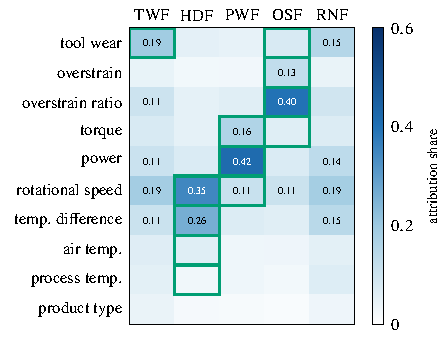
\includegraphics[width=0.82\columnwidth]{figures/attribution_heatmap.pdf}
\caption{Share of held-out attribution per feature on each mechanism's
observations (primary audit). Green outlines mark the expected sets $E_m$;
shares of at least 0.10 are printed.}
\label{fig:heatmap}
\end{figure}

\paragraph{TWF} Tool-wear failure is not aligned ($p_R=0.201$, $p_D=0.077$). Tool wear is its most important feature but receives only 19\% of the attribution, compared with 15\% under the null. The model also detects few of these failures. Held-out recall on TWF observations is 0.07, because the rule draws a random failure point inside a tool-wear window. Aligned attribution and successful detection are therefore separate properties. \Cref{sec:variants} examines how the TWF result depends on the attribution reference.

\section{Experimental Analysis}
\label{sec:analysis}

\Cref{sec:naive} examines whether the controls of the audit are necessary, \cref{sec:robust,sec:variants} study how robust its results are, \cref{sec:sweep,sec:scale} study shortcut detection, and \cref{sec:cwru} applies the audit to measured and process data.

\subsection{Need for Held-Out Explanations and a Retrained Null}
\label{sec:naive}

An audit should reject a model that has learned nothing, and it should not reward overfitting. A classifier trained on shuffled labels fails our alignment tests. If the same model is instead compared with random failure observations, all four mechanisms appear significant (adjusted $p=0.002$), because mechanism observations have unusual sensor values that receive large attributions in any case. Explaining training observations is also too optimistic. In-sample SHAP passes all four mechanisms, including TWF ($p=0.004$), and $R_{\mathrm{TWF}}$ rises from 0.19 to 0.35. In our experiments, held-out explanations and the retrained null prevented these misleading conclusions. The single shuffled-label model serves as a sanity check and is not a calibration of the false-positive rate.

\subsection{Robustness of the Verdicts}
\label{sec:robust}

\begin{table}[t]
\centering
\caption{Verdicts for selected audit variants: \checkmark~aligned,
$\times$~not aligned, \textbf{!}~flagged. All variants and full Holm-adjusted $p$-values are in the supplement.}
\label{tab:robust}
\footnotesize
\setlength{\tabcolsep}{4pt}
\begin{tabular}{@{}lrcccc@{}}
\toprule
Variant & $K$ & TWF & HDF & PWF & OSF \\
\midrule
\multicolumn{6}{@{}l}{\textit{Primary and null}} \\
Primary audit & 1000 & $\times$ & \checkmark & \checkmark & \checkmark \\
Seeds 1--4 (largest $p$) & 200 & $\times$ & \checkmark & \checkmark & \checkmark \\
Null re-tuned per permutation & 500 & $\times$ & \checkmark & \checkmark & \checkmark \\
\addlinespace[2pt]
\multicolumn{6}{@{}l}{\textit{Data and expected sets}} \\
Raw features only & 1000 & $\times$ & $\times$ & \checkmark & \checkmark \\
Label = OR of flags & 200 & $\times$ & \checkmark & \checkmark & \checkmark \\
$E_m$ without top trigger & 200 & $\times$ & \textbf{!} & \textbf{!} & \textbf{!} \\
\addlinespace[2pt]
\multicolumn{6}{@{}l}{\textit{Imbalance treatment}} \\
Class weights & 200 & $\times$ & \checkmark & \checkmark & \checkmark \\
Focal loss & 200 & \checkmark & \checkmark & \checkmark & \checkmark \\
SMOTE & 200 & $\times$ & $\times$ & \checkmark & \checkmark \\
\addlinespace[2pt]
\multicolumn{6}{@{}l}{\textit{Attribution (XGBoost)}} \\
Interventional, training bg. & 200 & \checkmark & \checkmark & \checkmark & \checkmark \\
\quad oversampled bg. & 200 & \checkmark & \checkmark & \checkmark & \checkmark \\
\quad failure-only bg. & 200 & \textbf{!} & $\times$ & $\times$ & \checkmark \\
Pairwise, nearest normal & 200 & \checkmark & \checkmark & \checkmark & \checkmark \\
Conditional group Shapley & 200 & \checkmark & \checkmark & \checkmark & \checkmark \\
LIME & 200 & \checkmark & \checkmark & $\times$ & \checkmark \\
\addlinespace[2pt]
\multicolumn{6}{@{}l}{\textit{Other models}} \\
Random forest, path TreeSHAP & 200 & $\times$ & \checkmark & \checkmark & \checkmark \\
MLP, KernelSHAP & 200 & $\times$ & $\times$ & $\times$ & $\times$ \\
MLP, Integrated Gradients & 200 & $\times$ & \checkmark & $\times$ & \checkmark \\
MLP, SmoothGrad & 200 & \textbf{!} & \checkmark & \checkmark & \checkmark \\
\addlinespace[2pt]
\multicolumn{6}{@{}l}{\textit{Sanity check}} \\
Permuted labels & 200 & $\times$ & $\times$ & $\times$ & $\times$ \\
\bottomrule
\end{tabular}

\end{table}

\Cref{tab:robust} summarizes selected variants; the supplement reports every variant and all three test results. Other seeds and the restriction to single-mechanism observations change nothing. Across five seeds, $R_m$ varies by at most 0.02 and every mechanism keeps the same three most attributed features; across seven interventional background sizes and seeds, it varies by at most 0.015. Re-tuning the hyperparameters on each of 500 permutations widens the null (the 95th percentile of $R_{\mathrm{OSF}}$ rises from 0.45 to 0.61) and leaves the results unchanged, although the relevant share of OSF moves closer to the threshold ($p=0.032$). Without the engineered features, the excess of $R_m$ over its null mean shrinks by 0.02--0.10 (HDF: from 0.15 to 0.06), PWF and OSF stay aligned, and HDF no longer passes the relevant-share test ($p=0.19$), consistent with difficulty representing the temperature-difference rule using separate temperature inputs. Label corrections change nothing, but the oversampler does matter. With SMOTE or ADASYN, HDF no longer passes the relevant-share test ($p=0.109$), and a focal-loss model trained without oversampling aligns TWF. When we removed the derived features or each mechanism's most attributed trigger from $E_m$, the affected mechanisms were flagged, and each flag named the omitted feature.

\paragraph{Supporting checks} Three further checks, which do not enter the audit decision, look at direction, feature removal, and statistical dependence. On mechanism observations, 97--99\% of the trigger features' attribution pushes toward failure (30--67\% on other failures). Retraining without a mechanism's raw trigger features cuts recall on its observations from 0.94 to 0.23 (HDF), 0.85 to 0.01 (PWF), and 0.95 to 0.23 (OSF). An HSIC check~\cite{daveiga2015global} between each input and the held-out prediction ranks a trigger feature first for all four mechanisms (rank correlation with the SHAP shares 0.27--0.90). These checks agree with the aligned results for HDF, PWF, and OSF. For TWF, HSIC ranks tool wear first even though the audit does not align the mechanism, which fits the reference dependence discussed next.

\subsection{Effect of the Model and Attribution Reference}
\label{sec:variants}

\paragraph{Beyond trees} HDF, PWF, and OSF stay aligned with interventional TreeSHAP and with a random forest, but other models and explainers behave less consistently. On the MLP (test F1 0.76), gradient explainers align some of the mechanisms (Integrated Gradients~\cite{sundararajan2017axiomatic}: HDF and OSF; DeepSHAP: HDF; SmoothGrad~\cite{smilkov2017smoothgrad}: HDF, PWF, and OSF), while KernelSHAP aligns none of them (\cref{fig:explainers}). Shuffled-label MLPs already place much attribution on the expected features ($R_{\mathrm{PWF}}$ null mean 0.60--0.63 versus 0.35 for XGBoost). Exact KernelSHAP with backgrounds of 100 or 500 observations or a k-means background gave the same results. LIME on XGBoost aligns HDF, OSF, and TWF, but not PWF ($p_D=0.16$). LIME explains failure probability, whereas the XGBoost SHAP and MLP attribution comparisons use logits; differences therefore need not arise from the explainer alone.

\begin{figure}[t]
\centering
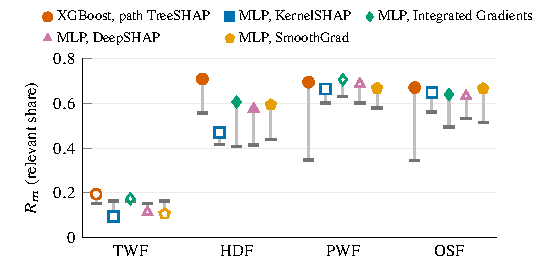
\includegraphics[width=\columnwidth]{figures/explainer_dependence.pdf}
\caption{Relevant share of each mechanism under XGBoost with path-dependent
TreeSHAP and an MLP with four explainers (markers; filled: aligned). Bars mark
each pipeline's own shuffled-label null mean, which is higher for the MLP on HDF, PWF, and OSF.}
\label{fig:explainers}
\end{figure}

\begin{figure}[t]
\centering
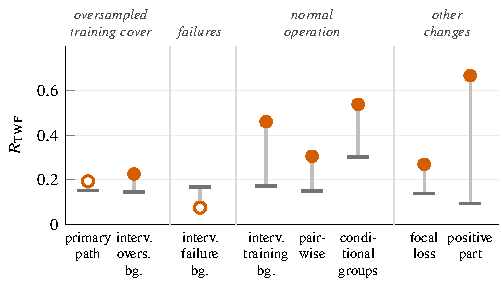
\includegraphics[width=\columnwidth]{figures/twf_reference.pdf}
\caption{Relevant share of TWF (circles; filled: aligned) under attribution
formulations grouped by the reference distribution against which attributions
are measured; bars mark each variant's own shuffled-label null mean.}
\label{fig:twfref}
\end{figure}

\paragraph{TWF and the reference distribution} TWF fails with path-dependent TreeSHAP but passes with interventional TreeSHAP for every background size and seed (\cref{fig:twfref}). Tool wear is correlated with the overstrain features overall (Spearman 0.92), but only 0.13 on TWF observations. The raw features alone show the same change, and summing path-dependent SHAP over groups of correlated features does not align TWF either. These checks suggest that correlation alone does not explain the difference, and the comparisons point to the reference distribution instead. Path-dependent TreeSHAP weights paths by the cover of the oversampled training data. An interventional background drawn from that data lowers $R_{\mathrm{TWF}}$ toward the path-dependent value, and a failure-only background removes the alignment. All tested normal-operation references align TWF. These are the interventional training background (97\% non-failures), the nearest normal observation~\cite{xu2025pairwise}, and exact conditional Shapley values of feature groups~\cite{aas2021explaining} for kernel bandwidths between 0.15 and 0.6 (at 0.6, where the kernel averages over most of the data, the other mechanisms lose alignment). A focal-loss model without oversampling and the failure-pushing part of path-dependent SHAP also align TWF. With a recall of 0.07, the absolute attribution of TWF observations is dominated by features that argue against failure. \Cref{fig:twfexample} shows this for a single TWF observation (tool wear 215~min, predicted failure probability 0.006), chosen because its path-dependent tool-wear share of 0.20 is closest to the TWF mean. Path-dependent TreeSHAP gives tool wear a positive contribution, but it assigns larger negative contributions to rotational speed, torque, and process temperature. The oversampled training data are balanced between failures and non-failures, and against this reference ordinary operating values look like evidence against failure. Measured against normal operation, the same model gives tool wear 0.47 of the absolute attribution and the other features little.

\begin{figure}[t]
\centering
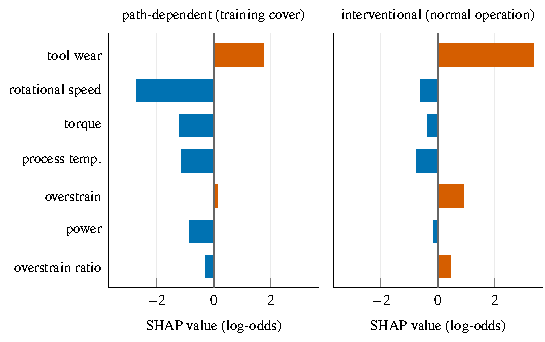
\includegraphics[width=\columnwidth]{figures/twf_example.pdf}
\caption{Signed SHAP values for one TWF observation from the same held-out
model under two reference distributions. Orange pushes toward failure, blue
away from it.}
\label{fig:twfexample}
\end{figure} These results suggest that the TWF result reflects the reference more than the model's use of tool wear, although they do not prove it. For questions about abnormal operation, we recommend a stated normal-operation reference.

\subsection{Detecting a Planted Shortcut}
\label{sec:sweep}

\begin{figure}[t]
\centering
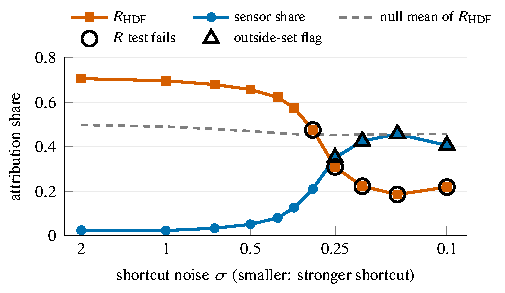
\includegraphics[width=\columnwidth]{figures/shortcut_sweep_tikz.pdf}
\caption{Planted shortcut: as the sensor's noise decreases, its share of HDF
attribution rises and $R_{\mathrm{HDF}}$ falls. Circles: relevant-share test
fails; triangles: outside-set test flags the sensor.}
\label{fig:sweep}
\end{figure}

\Cref{fig:sweep} shows two different reactions of the audit. Weak shortcuts ($\sigma\geq0.35$, at most 13\% of HDF attribution) leave HDF aligned. A moderate shortcut ($\sigma=0.30$, 21\%) removes the alignment because the relevant-share test fails, but no feature is flagged. Stronger shortcuts ($\sigma\leq0.25$, at least 35\%) are flagged by the outside-set test, which names the sensor. Test F1 stays between 0.84 and 0.92 in all settings, and PWF and OSF remain aligned. These strengths apply to this particular sensor and sample size (\cref{sec:scale}). Two alternative outside-set statistics, one standardized against the null alone and one computed on failure-pushing attribution, did not flag the sensor earlier (see the supplement). When the planted signal is split over three sensors with independent noise, the model spreads attribution over them. At $\sigma=0.35$ they receive 38\% of HDF attribution together, more than the single sensor flagged at $\sigma=0.25$, but at most 14\% each. HDF is then not aligned, yet no feature is flagged until $\sigma=0.25$ (54\% together). Because $C_m$ takes the maximum over single features, a shortcut spread over several inputs is harder to name.

\subsection{Effect of Sample Size}
\label{sec:scale}

\begin{table}[t]
\centering
\caption{Verdicts on generated data of increasing size ($K=200$): numbers
of runs aligned (A), not aligned (N), and flagged (F). Share: planted
sensor's share of HDF attribution; Min.: minutes per full audit on eight cores.}
\label{tab:scale}
\footnotesize
\setlength{\tabcolsep}{3pt}
\begin{tabular}{@{}rcccccccccr@{}}
\toprule
& & & & \multicolumn{3}{c}{HDF verdicts} & \multicolumn{3}{c}{TWF verdicts} & \\
\cmidrule(lr){5-7}\cmidrule(lr){8-10}
$n$ & $\sigma$ & Runs & Share & A & N & F & A & N & F & Min. \\
\midrule
10{,}000 & none & 3 & -- & 3 & 0 & 0 & 0 & 3 & 0 & 3 \\
 & 0.35 & 3 & 0.158 & 1 & 2 & 0 & 0 & 3 & 0 & 3 \\
 & 0.25 & 3 & 0.390 & 0 & 0 & 3 & 0 & 3 & 0 & 3 \\
\addlinespace
30{,}000 & none & 3 & -- & 3 & 0 & 0 & 0 & 2 & 1 & 7 \\
 & 0.35 & 3 & 0.128 & 3 & 0 & 0 & 0 & 3 & 0 & 6 \\
 & 0.25 & 3 & 0.346 & 0 & 0 & 3 & 0 & 2 & 1 & 7 \\
\addlinespace
100{,}000 & none & 3 & -- & 3 & 0 & 0 & 0 & 1 & 2 & 17 \\
 & 0.35 & 3 & 0.100 & 3 & 0 & 0 & 0 & 2 & 1 & 19 \\
 & 0.25 & 3 & 0.315 & 0 & 0 & 3 & 0 & 2 & 1 & 19 \\
\addlinespace
300{,}000 & none & 1 & -- & 1 & 0 & 0 & 0 & 1 & 0 & 52 \\
 & 0.35 & 1 & 0.063 & 1 & 0 & 0 & 0 & 1 & 0 & 59 \\
 & 0.25 & 1 & 0.271 & 0 & 0 & 1 & 0 & 0 & 1 & 61 \\
\bottomrule
\end{tabular}

\end{table}

More data kept several alignment results stable, but it did not make shortcut diagnosis reliable (\cref{tab:scale}). Without a sensor, HDF, PWF, and OSF are aligned at every size, and TWF never is. The strong sensor ($\sigma=0.25$) is flagged in all ten runs, including at $3\cdot10^5$ observations, where the relevant-share test alone would pass ($R_{\mathrm{HDF}}=0.472$, above the null's 95th percentile of 0.417). As the null narrows with more data, a model can beat the shuffled-label pipelines while relying heavily on a misleading feature, and in this case only the outside-set test changes the result. The weaker sensor ($\sigma=0.35$) removes HDF alignment in two of three runs at $10^4$ observations and in none at larger sizes. TWF is flagged in 7 of 30 runs from $3\cdot10^4$ observations on, on air or process temperature with excesses of 0.03--0.05. The generator draws temperatures independently of tool life, so these flags do not reflect the physical rule. They may still reflect a real dependence of the model on temperature, which the audit reports correctly. In all our experiments, these small excesses (at most 0.047) were separated from the planted shortcuts, the gain shortcut, and the omitted triggers (at least 0.165) by a minimum excess of 0.05. We chose this cutoff after seeing the results, so it is only exploratory. Applied as a rule, it would remove these TWF flags and the TEP IDV5 flags (\cref{sec:cwru}) and keep every planted-sensor, gain-shortcut, and omitted-trigger flag. The largest size has a single generation seed, and the findings at this size should be read as examples. With fixed hyperparameters, a five-fold audit requires $5(K+1)$ model fits; hyperparameter searches require additional fits. In timing checks, one cross-fitted run took 1.3, 31, and 115~seconds on one core at $10^4$, $3\cdot10^5$, and $10^6$ observations.

\subsection{Application to Measured and Process Data}
\label{sec:cwru}

\begin{table}[t]
\centering
\caption{Audit on CWRU bearing data ($K=1{,}000$) and simulated Tennessee
Eastman process data ($K=200$); Holm-adjusted $p$.}
\label{tab:cwru}
\footnotesize
\setlength{\tabcolsep}{2.5pt}
\begin{tabular}{@{}llrrrrrrl@{}}
\toprule
Data & Fault & $R_m$ & $p$ & $D_m$ & $p$ & $C_m$ & $p$ & Verdict \\
\midrule
CWRU & Inner & 0.440 & 0.004 & 0.190 & 0.030 & 0.065 & 1.000 & aligned \\
 & Ball & 0.133 & 0.773$^{\times}$ & 0.036 & 0.211$^{\times}$ & 0.051 & 1.000 & not aligned \\
 & Outer & 0.392 & 0.003 & 0.131 & 0.027 & 0.042 & 1.000 & aligned \\
\addlinespace
+ gain & Inner & 0.394 & 0.018 & 0.168 & 0.054$^{\times}$ & 0.063 & 0.989 & not aligned \\
 & Ball & 0.105 & 0.948$^{\times}$ & 0.029 & 0.547$^{\times}$ & 0.020 & 0.989 & not aligned \\
 & Outer & 0.269 & 0.018 & 0.050 & 0.547$^{\times}$ & 0.165 & 0.006$^{\dagger}$ & flagged \\
\addlinespace
TEP & IDV4 & 0.747 & 0.010 & 0.568 & 0.010 & 0.000 & 1.000 & aligned \\
 & IDV5 & 0.221 & 0.010 & 0.164 & 0.010 & 0.026 & 0.010$^{\dagger}$ & flagged \\
\bottomrule
\end{tabular}

\end{table}

These datasets show how the audit can be applied beyond documented rules (\cref{tab:cwru}). They do not test cross-domain transfer or validate the audit on operating plants.

\paragraph{CWRU} The forest classifies all 36 held-out recordings correctly (window accuracy 0.99). Inner- and outer-race attribution concentrates on their defect frequencies ($R_m=0.44$ and 0.39 against null means of 0.23 and 0.15) and is aligned. Ball faults are not aligned with bands of $\pm0.15$ orders (share 0.13, below the null mean of 0.17), but they are aligned with bands of $\pm0.3$ orders, and bands of $\pm0.05$ orders remove the inner-race specificity ($p_D=0.09$). The results therefore depend on how the bands are defined, and perfect classification alone does not show that the feature map is physically adequate. With the gain shortcut, every recording is still classified correctly, yet the outer-race share on log-RMS rises from 0.13 to 0.38 and its defect-band share falls from 0.39 to 0.27 (\cref{fig:cwru}). The outside-set test flags this shift ($C_m=0.165$, $p=0.006$).

\begin{figure}[t]
\centering
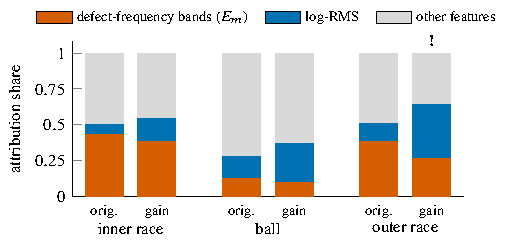
\includegraphics[width=\columnwidth]{figures/cwru_shares.pdf}
\caption{CWRU: share of attribution on the defect-frequency bands, on log-RMS,
and on the other features for each fault, on the original recordings and with
the acquisition-gain shortcut. !: flagged by the outside-set test.}
\label{fig:cwru}
\end{figure}

\paragraph{TEP} IDV4 is detected in every sample and aligned (75\% of its attribution on the reactor-cooling loop, null mean 6\%). IDV5 is our clearest example of an ambiguous flag. For the condenser disturbance, IDV5 recall is 0.39; the pooled fault-active-class F1 across both fault types is 0.76, consistent with compensation by the controllers. Attribution concentrates on the disturbed loop (0.22 versus 0.06), but the outside-set test flags a small excess (0.026) on the E-feed valve. We suspect a downstream control response that the three-variable map does not cover, but our data cannot separate this from a shortcut, and the flag has to be inspected. When 30-minute means and changes are added as inputs, IDV5 recall rises to 0.86 and its loop share to 0.54. The E-feed excess shrinks to 0.011 but is still flagged. The LSTM on 30-minute sequences gives pooled fault-active-class F1 0.91 and IDV5 recall 0.81. IDV4 is aligned, and IDV5 passes both alignment tests but is flagged again, this time on the D-feed valve (excess 0.011). Both models flag outside-set attribution, although on different feed valves. This does not distinguish downstream process responses from shortcut reliance. With the rotated-label null, the verdicts of the static and the 30-minute-feature models are unchanged.

\subsection{Audit-Component Ablations}
\label{sec:compare}

\Cref{tab:compare} summarizes selected diagnostic checks of reduced audit designs: rejecting a model trained on shuffled labels (\cref{sec:naive}), avoiding the optimistic in-sample TWF result (\cref{sec:naive}), and detecting the strong shortcut at $3\cdot10^5$ observations (\cref{sec:scale}). Among designs producing statistical verdicts, each reduced design misses at least one selected check. Global SHAP rankings do not produce such verdicts. The full audit passes these three checks; this is an ablation summary, not a general comparative performance evaluation.

\begin{table}[t]
\centering
\begin{threeparttable}
\caption{Audit-component ablations on three selected diagnostic checks.}
\label{tab:compare}
\footnotesize
\setlength{\tabcolsep}{3pt}
\begin{tabular}{@{}l>{\centering\arraybackslash}b{1.25cm}>{\centering\arraybackslash}b{1.25cm}>{\centering\arraybackslash}b{1.25cm}@{}}
\toprule
Design & Rejects shuffled labels & Avoids in-sample TWF pass & Detects shortcut at $3\cdot10^5$ \\
\midrule
Global SHAP ranking~\cite{milling2025shap} & -- & -- & -- \\
Naive null & No & No & No \\
In-sample SHAP & Yes & No & No \\
Relevant share $R_m$ only & Yes & Yes & No \\
\addlinespace
\textbf{Full audit} & \textbf{Yes} & \textbf{Yes} & \textbf{Yes} \\
\bottomrule
\end{tabular}
\begin{tablenotes}[flushleft]
\footnotesize
\item ``--'': no statistical result. The naive null passes all four
mechanisms ($p=0.002$); in-sample SHAP, tested against the shuffled-label
null, passes TWF ($p=0.004$) and misses the shortcut ($p_C=0.06$).
\end{tablenotes}
\end{threeparttable}
\end{table}

\section{Discussion and Limitations}
\label{sec:limits_future}

The audit results hold for a stated configuration and depend on the attribution reference (TWF), the oversampler and engineered features (HDF), the model and explainer, and the expected sets (CWRU ball faults). A flag on its own cannot tell a missing trigger, a downstream effect, and a shortcut apart, as the TEP case IDV5 shows. The outside-set test missed weak planted shortcuts and shortcuts spread over several sensors, and it flagged small excesses at large $n$, and the shuffled-label reference is a sanity check and not a calibrated false-positive rate. Because AI4I and TEP are simulated and CWRU uses laboratory faults, we can only establish agreement with documented rules and physics, and not with verified causes in operating plants.

For practitioners we suggest the following defaults. Fix $E_m$ before the audit, explain only held-out observations, and refit the full pipeline for $K\geq200$ shuffled-label nulls ($K\geq500$ when an adjusted $p$ lies near $\alpha$; with $M$ mechanisms, $K\geq M/\alpha$). Measure attributions against normal operation for questions about abnormal behaviour and report the reference. Call a mechanism aligned only when both $R_m$ and $D_m$ pass, report effect sizes with every verdict, treat outside-set excesses below about 0.05 as exploratory, and inspect every flag. The supplement expands these defaults into a checklist.

Future work should complete and test mechanism maps, validate thresholds for effect sizes, develop more sensitive outside-set statistics, compare conditional Shapley estimators based on learned generative models, and apply the audit to plant data with recorded failure causes.


\section{Conclusion}
\label{sec:conclusion}

We proposed a mechanism-level audit comparing held-out attributions with retrained shuffled-label pipelines. On AI4I~2020, a tuned XGBoost model passed for three of four mechanisms. Controlled examples exposed misleading passes without the audit controls and missed weak shortcuts. Results across datasets depended on the attribution reference and mechanism map. These choices should be fixed and reported alongside effect sizes and flagged features. A passing result supports attribution concentration under the stated configuration, without certifying physical correctness. Outside-set flags require investigation.

\bibliographystyle{IEEEtran}
\bibliography{refs}

\end{document}
